\begin{figure}[H]
\centering
\begin{tikzpicture}[scale=0.95]
% 3D 坐标轴（斜投影）
\draw[->] (0,0,0)--(4.2,0,0) node[right]{$2$};
\draw[->] (0,0,0)--(0,3.4,0) node[above]{$3$};
\draw[->] (0,0,0)--(-1.6,-1.3,0) node[below left]{$1$};
% 刻度标签
\node[font=\scriptsize,below] at (2.2,0,0){$1$};
\node[font=\scriptsize,below] at (3.2,0,0){$2$};
\node[font=\scriptsize,left] at (0,1.2,0){$1$};
\node[font=\scriptsize,left] at (0,2.2,0){$2$};
\node[font=\scriptsize,left] at (0,3.0,0){$3$};
\node[font=\scriptsize,above left] at (-0.8,-0.65,0){$1$};
\node[font=\scriptsize,above left] at (-1.3,-1.05,0){$2$};
% 向量 y1 = (4,-1,3)
\draw[->,line width=1.1pt] (0,0,0)--(3.05,-0.85,0) coordinate (Y1);
\node[right,font=\small] at (3.05,-0.85,0) {$\mathbf{y}_{1}$};
% 向量 y2 = (1,3,5)
\draw[->,line width=1.1pt] (0,0,0)--(0.55,2.6,0) coordinate (Y2);
\node[right,font=\small] at (0.55,2.6,0) {$\mathbf{y}_{2}$};
% 虚线投影
\draw[dashed] (3.05,-0.85,0)--(3.05,0,0);
\draw[dashed] (3.05,-0.85,0)--(0,-0.85,0);
\draw[dashed] (0.55,2.6,0)--(0.55,0,0);
\draw[dashed] (0.55,2.6,0)--(0,2.6,0);
\end{tikzpicture}
\caption{数据矩阵 $\mathbf{X}$ 作为 $n=3$ 维空间中 $p=2$ 个向量的图形}
\end{figure}

可惜, 我们局限于只能在三维中使对象形象化, 因此, 数据矩阵 $\mathbf{X}$ 的 $n$ 维表示法对于 $n>3$ 似乎不会是特别有用. 然而, 对任何 3 个向量描述的几何关系和相联系的统计概念, 不论它们的维数是多少仍然是有效的. 这是因为, 3 个向量, 即使是 $n$ 维的, 可以生成不超过 3 维的空间, 正如任意多个分量的 2 个向量必定在一个平面中. 通过选择一个适当的三维透视——即 $n$ 维空间中包含 3 个感兴趣向量的那一部分——得到了保持其长度和角度的一个视图. 这样, 在正确选择了轴的情况下, 利用任意维数 $n$ 的 2 个或 3 个向量, 说明某些代数统计概念是可能的. 由于轴的具体选择与几何形状是不相关的, 我们总是标明坐标轴 1,2 和 3.

给出求样本均值方法的几何解释是可能的. 首先, 定义 $n\times1$ 向量 $\mathbf{1}_{n}'=[1,1,\cdots,1]$ (为了简化符号, 当向量 $\mathbf{1}_{n}$ 的维数从上下文可以清楚看出时, 下标 $n$ 可省略). 向量 $\mathbf{1}$ 与 $n$ 个坐标轴的每一个形成等角, 这样向量 $(1/\sqrt{n})\mathbf{1}$ 在等角方向上为单位长度. 设向量 $\mathbf{y}_{j}'=[x_{1j},x_{2j},\cdots,x_{nj}]$. 由\hyperref[eq:2-8]{式(2-8)}, $\mathbf{y}_{j}$ 在单位向量 $(1/\sqrt{n})\mathbf{1}$ 上的投影是,
\phantomsection\label{eq:3-3}
\begin{equation}
\mathbf{y}_{j}'\Bigl(\frac{1}{\sqrt{n}}\mathbf{1}\Bigr)\frac{1}{\sqrt{n}}=\frac{x_{1j}+x_{2j}+\cdots+x_{nj}}{n}\mathbf{1}=\bar{x}_{j}\mathbf{1}
\tag{3-3}
\end{equation}
即样本均值 $\bar{x}_{j}=(x_{1j}+x_{2j}+\cdots+x_{nj})/n=\mathbf{y}_{j}'\mathbf{1}/n$ 对应于 $\mathbf{1}$ 的倍数, 该倍数给出 $\mathbf{y}_{j}$ 在由 $\mathbf{1}$ 确定的直线方向上的投影.

更进一步, 对每个 $\mathbf{y}_{j}$ 有分解

\begin{center}
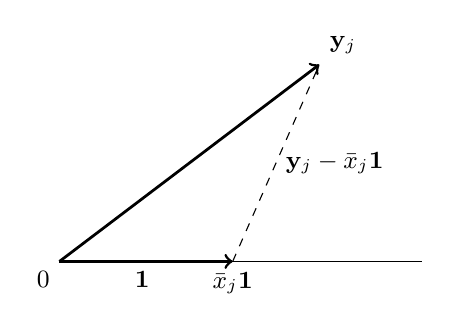
\begin{tikzpicture}[scale=1.0]
\draw (0,0)--(4.6,0);
\draw[->,line width=1.0pt] (0,0)--(3.3,2.5) node[above right,font=\small]{$\mathbf{y}_{j}$};
\draw[->,line width=1.0pt] (0,0)--(2.2,0) node[below,font=\small]{$\bar{x}_{j}\mathbf{1}$};
\draw[dashed] (2.2,0)--(3.3,2.5);
\node[right,font=\small] at (2.75,1.25){$\mathbf{y}_{j}-\bar{x}_{j}\mathbf{1}$};
\node[below left,font=\small] at (0,0){$0$};
\node[below,font=\small] at (1.05,0){$\mathbf{1}$};
\end{tikzpicture}
\end{center}

其中 $\bar{\mathbf{x}}_{j}\mathbf{1}$ 垂直于 $\mathbf{y}_{j}-\bar{x}_{j}\mathbf{1}$. 偏差 (或均值修正) 向量为
\phantomsection\label{eq:3-4}
\begin{equation}
\mathbf{d}_{j}=\mathbf{y}_{j}-\bar{x}_{j}\mathbf{1}=\begin{bmatrix}x_{1j}-\bar{x}_{j}\\x_{2j}-\bar{x}_{j}\\\vdots\\x_{nj}-\bar{x}_{j}\end{bmatrix}
\tag{3-4}
\end{equation}
